%----------------------------------------------------------------------------------------
%	PACKAGES AND OTHER DOCUMENT CONFIGURATIONS
%----------------------------------------------------------------------------------------

\documentclass[twoside,twocolumn,a4paper]{article}

\usepackage{blindtext} % Package to generate dummy text throughout this template 

\usepackage{mhchem}

\usepackage{gensymb}

\usepackage[super]{natbib}

\usepackage[T1]{fontenc} % Use 8-bit encoding that has 256 glyphs

\usepackage{lmodern}

\usepackage[hyphenbreaks]{breakurl}

\usepackage[hyphens]{url}

%\usepackage[super,sort&compress]{natbib}
%\usepackage{natbib}
%\setlength{\bibsep}{0.0pt}

\usepackage{graphicx}

\linespread{1.05} % Line spacing - Palatino needs more space between lines
\usepackage{microtype} % Slightly tweak font spacing for aesthetics

\usepackage[spanish]{babel} % Language hyphenation and typographical rules

\usepackage[numbib,notlof,notlot,nottoc]{tocbibind} % Shows bibliography as a section

\usepackage[hmarginratio=1:1,top=32mm,columnsep=20pt]{geometry} % Document margins

\usepackage[hang, small,labelfont=bf,up,textfont=up]{caption} % Custom captions under/above floats in tables or figures

\usepackage[section]{placeins}

\usepackage{float}

\usepackage{booktabs} % Horizontal rules in tables

\usepackage{enumitem} % Customized lists

\setlist[itemize]{noitemsep} % Make itemize lists more compact

\usepackage{abstract} % Allows abstract customization

\renewcommand{\abstractnamefont}{\normalfont\bfseries} % Set the "Abstract" text to bold

\usepackage{fancyhdr} % Headers and footers
\pagestyle{fancy} % All pages have headers and footers
\fancyhead{} % Blank out the default header
\fancyfoot{} % Blank out the default footer
\fancyhead[C]{Laboratorio 4 $\bullet$ Informe 3 $\bullet$ Grupo 3: Poggi, R\'ios Ch\'avez} % Custom header text
\fancyfoot[C]{\thepage} % Custom footer text

\usepackage{titling} % Customizing the title section

\usepackage{hyperref} % For hyperlinks in the PDF

%----------------------------------------------------------------------------------------
%	TITLE SECTION
%----------------------------------------------------------------------------------------

\setlength{\droptitle}{-4\baselineskip} % Move the title up

\pretitle{\begin{center}\LARGE\bfseries} % Article title formatting
\posttitle{\end{center}} % Article title closing formatting
\title{Piezoel\'ectrico} % Article title
\author{%
\textsc{Ignacio Poggi} \\[1ex] % Your name
\normalsize \href{mailto:ignaciop.3@gmail.com}{ignaciop.3@gmail.com} % Your email address
\and % Uncomment if 2 authors are required, duplicate these 4 lines if more
\textsc{Carlos R\'ios Ch\'avez} \\[1ex] % Second author's name
\normalsize \href{mailto:carlos_rios_ch@hotmail.com}{carlos\_rios\_ch@hotmail.com} % Second author's email address
}



\date{Grupo 3 - Laboratorio 4, C\'atedra Schmiegelow - Departamento de F\'isica, Facultad de Ciencias Exactas y Naturales, Universidad de Buenos Aires \newline \\ \today} % Leave empty to omit a date
\renewcommand{\maketitlehookd}{%
\begin{abstract}
\noindent En este trabajo se estudi\'o el comportamiento de un material piezoel\'ectrico de cuarzo sometido a una se\~nal el\'ectrica. Mediante el modelado de este material por un circuito RLC y el an\'alisis de los datos recolectados utilizando varios m\'etodos, se obtuvieron las frecuencias de resonancia y antirresonancia, el factor de m\'erito $Q$ y los par\'ametros $R$, $L$ y $C$ del circuito equivalente.
\end{abstract}
}

%----------------------------------------------------------------------------------------

\begin{document}
\maketitle

% Print the title

%----------------------------------------------------------------------------------------
%	ARTICLE CONTENTS
%----------------------------------------------------------------------------------------

\section{Introducci\'on}



El efecto piezoel\'ectrico describe la capacidad de dichos materiales minerales, como el cuarzo, de producir una carga el\'ectrica en respuesta a un esfuerzo mec\'anico aplicado; o de manera inversa, deformarse al estar expuestos a un campo el\'ectrico. \newline

\par
Como consecuencia de este comportamiento, los s\'olidos piezoel\'ectricos pueden resonar a ciertas frecuencias que dependen de la naturaleza del mismo y de su forma geom\'etrica. Hay ciertas frecuencias para las cuales la transferencia de energ\'ia electromec\'anica es m\'axima (resonancia), y otras para las cuales \'esta es m\'inima (antirresonancia). En este sentido, el cristal piezoel\'ectrico se comporta de manera an\'aloga a un circuito RLC en serie, para el cual su din\'amica se describe mediante la siguiente ecuaci\'on diferencial \cite{eq:oderlc}:

\begin{equation}
\label{eq:oderlc}
L\frac{d^{2}i}{dt^{2}} + R\frac{di}{dt} + \frac{1}{C}i = \frac{dV}{dt}
\end{equation}

donde $R$, $L$, $C$ y $V$ son la resistencia, inductancia, capacitancia y voltaje del circuito, respectivamente. \newline


\par
Dado que en el piezoel\'ectrico estudiado hay dos placas de metal adosadas a dos de sus lados, que funcionan como una capacidad adicional junto con el cristal; hay que tener en cuenta en el circuito el\'ectrico equivalente una capacidad $C_{2}$ en paralelo con el piezoel\'ectrico, como muestra la Figura \ref{fig:esquemapzt}.

\begin{figure}[H]
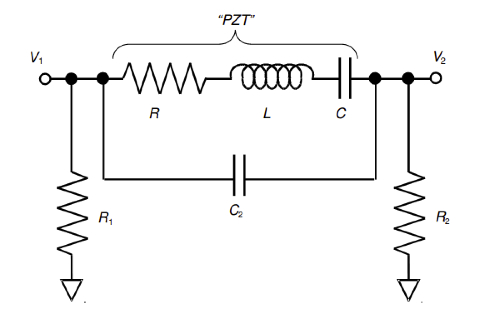
\includegraphics[width=\linewidth]{esquemapzt.jpg}
\caption{Diagrama del circuito RLC equivalente para el piezoel\'ectrico de cuarzo. Se muestra la capacidad adicional $C_{2}$ introducida por las placas de metal agregadas al cristal; $R_{1}$ y $R_{2}$ resistencias arbitrarias y los voltajes de entrada y salida $V_{1}$ y $V_{2}$, respectivamente.}
\label{fig:esquemapzt}
\end{figure}

Gracias al modelado del material de cuarzo como un circuito RLC, podemos calcular algunas de sus propiedades para poder caracterizarlo, siendo de nuestro inter\'es los par\'ametros $R$, $L$, $C$ y $C_{2}$ del mismo. Para eso, veamos algunas propiedades de los circuitos mencionados, por ejemplo su admitancia, dada por la siguiente ecuaci\'on\cite{eq:props}:

\begin{equation}
\label{eq:admitancia}
Y = \frac{1}{Z} = \frac{R}{R^{2} + \Omega^{2}} + j(\omega C_{2} - \frac{\Omega}{R^{2} + \Omega^{2}})
\end{equation}

siendo $Z$ la impedancia y $\Omega = \omega L - \frac{1}{\omega C}$.

La transferencia de energ\'ia del circuito est\'a dada por: 

\begin{equation}
\label{eq:transferencia}
T = \frac{|V_{2}|}{|V_{1}|} = \frac{R_{2}}{R_{2} + Z}
\end{equation}

donde $R_{2}$ es una resistencia arbitraria en el circuito, $V_{1}$ y $V_{2}$ los voltajes de entrada y salida respectivamente.
Evaluando la transferencia en la frecuencia de resonancia $\omega_{r}$ del sistema se obtiene la siguiente ecuaci\'on, la cual nos permitir\'a calcular la resistencia $R$:

\begin{equation}
\label{eq:transferenciar}
T(\omega_{r}) = \frac{R_{2}}{R_{2} + R}
\end{equation}

\par
El par\'ametro $L$ se define a partir del c\'alculo del factor de calidad  $Q$ del cristal. Este factor est\'a dado por la ecuaci\'on:

\begin{equation}
\label{eq:merito}
Q = \frac{\omega_{r}}{\Delta \omega} = \frac{\omega_{r}L}{R_{2} + R}
\end{equation}

donde $\Delta \omega$ es el ancho de la campana de resonancia. \newline

\par
Por \'ultimo, se pueden obtener los valores para la frecuencia de resonancia $\omega_{r}$ y antirresonancia $\omega_{a}$ experimentalmente mediante las siguientes ecuaciones, teniendo en cuenta que $C$ es muy peque\~no comparado con $C_{2}$:

\begin{equation}
\label{eq:wr}
\omega_{r} = \frac{1}{\sqrt{LC}}
\end{equation}

\begin{equation}
\label{eq:wa}
\omega_{a} = \sqrt{\frac{1}{L}(\frac{1}{C} + \frac{1}{C_{2}})}
\end{equation}

%------------------------------------------------

\section{Dispositivo experimental}

Los instrumentos de laboratorio utilizados fueron:
\begin{itemize}
\item 
\label{Laser} PC con software MATLAB para la adquisici\'on y an\'alisis de los datos.
\item Generador de funciones Tektronix AFG3021B.
\item Osciloscopio Tektronix TDS1002B.
\item Amplificador Lock-In Stanford Research Systems SR830DSP, con interfaz GPIB.
\item Cables BNC.
\item Cristal piezoel\'ectrico de cuarzo.
\end{itemize}


En esta experiencia, se trabaj\'o con un cristal piezoel\'ectrico de base cuadrada, cortado a +5 \degree respecto de uno de sus ejes; contenido en una base cerrada de acr\'ilico. En dos de las caras del cristal, se encontraban dispuestos electrodos de metal, cada uno con un alambre soldado, cada uno de los cuales estaban en serie con una resistencia de 10 K$\Omega$. En la siguiente figura se puede ver un esquema del dispositivo utilizado:

\begin{figure}[H]
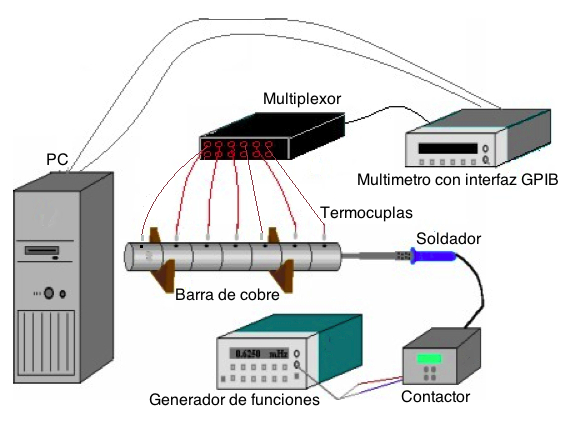
\includegraphics[width=\linewidth]{dispexp.jpg}
\caption{Esquema del dispositivo experimental utilizado. En primera instancia, en lugar del amplificador se dispuso un osciloscopio.}
\label{fig:dispexp}
\end{figure}

En uno de los alambres mencionados, se utiliz\'o el generador de funciones para aplicar una se\~nal de entrada $V_{1}$ de amplitud 2 Vpp y frecuencia variable. Luego, sobre el otro alambre se registr\'o la se\~nal de salida $V_{2}$, en primera instancia con el osciloscopio y luego con el amplificador lock-in. Con \'este \'ultimo tambi\'en se obtuvo la diferencia de fase entre la se\~nal de entrada y la de salida. Cabe aclarar que, para poder establecer una se\~nal de referencia requerida por el amplificador lock-in, se conect\'o una de las salidas del generador de funciones con la entrada de referencia del amplificador.


Finalmente, se conectaron el osciloscopio (mediante cable USB) y el amplificador (mediante interfaz GPIB) a una PC con software MATLAB,    con el cual se ejecut\'o un script para poder recolectar y analizar los datos enviados por los equipos mencionados.

%------------------------------------------------
\section{Resultados y an\'alisis}

Para poder estimar la frecuencia de resonancia del cristal de cuarzo, en primer lugar se utiliz\'o el generador de funciones para realizar manualmente un barrido de frecuencias y el osciloscopio para poder visualizar la amplitud de la onda y obtener la campana de resonancia de dicho cristal, como muestra la siguiente figura:

\begin{figure}[H]
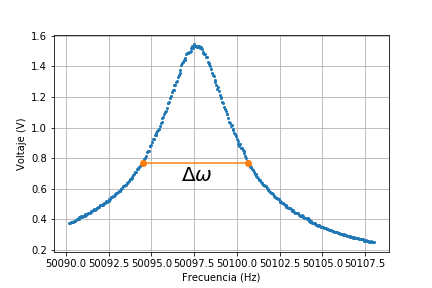
\includegraphics[width=\linewidth]{detallecampanaOSC.png}
\caption{Campana de resonancia obtenida mediante un barrido de frecuencias manual con el osciloscopio.}
\label{fig:detallecampanaOSC}
\end{figure}

Luego, se pudo calcular la frecuencia de resonancia y el ancho de la campana, dando como resultado $\omega_{r}$ = (50108 $\pm$ 7) Hz y $\Delta \omega$ = (6,15 $\pm$ 0,10) Hz respectivamente. Con estos datos, se obtuvo el factor de m\'erito del circuito, $Q$ = 8147 $\pm$ 70. \newline

\par
Adem\'as, se intent\'o calcular la frecuencia de antirresonancia utilizando este m\'etodo; pero al aumentar la escala en el gr\'afico anterior en la zona correspondiente a dicha frecuencia (50,025 kHz $< \omega_{a} <$ 50,03 kHz), notamos que por la baja resoluci\'on del osciloscopio no se pudo obtener un valor confiable para $\omega_{a}$. \newline


\par
Posteriormente se analizaron los datos obtenidos por el amplificador lock-in. Se realizaron varios barridos de frecuencia con distintos niveles de resoluci\'on en la variaci\'on de la frecuencia, procurando que el barrido sea fino en los rangos que m\'as nos interesaron, es decir cerca a la resonancia y la antirresonancia, previamente estimadas. Se trabaj\'o con todas las mediciones en una sola base de datos y para determinar la frecuencia de resonancia se utilizaron tres m\'etodos, el primero consisti\'o en ajustar la curva de voltaje a una curva lorentziana, ajuste del cual se obtuvo que $\omega_{r}$ = (50097,85 $\pm$ 0,01) Hz (la bondad del ajuste fue $R^{2}$ = 0,992), como muestra la Figura \ref{fig:ajuste}:


\begin{figure}[H]
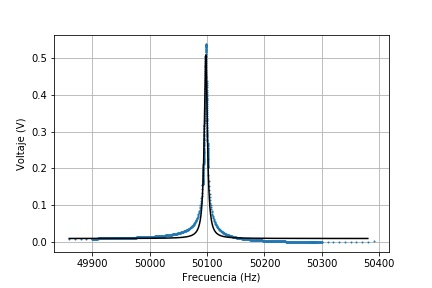
\includegraphics[width=\linewidth]{ajuste.jpg}
\caption{Ajuste a una funci\'on lorentziana del voltaje con respecto a la frecuencia.}
\label{fig:ajuste}
\end{figure}


El segundo m\'etodo consisti\'o en encontrar la frecuencia para la cual la transferencia de energ\'ia es m\'axima considerando que la transferencia es directamente proporcional al voltaje registrado,  Figura \ref{fig:detalleRESamp}. Se obtuvo que $\omega_{r}$ = (50097,9 $\pm$ 0,3) Hz y en el caso de la antirresonancia se determin\'o la frecuencia en la cual la transferencia de energ\'ia es m\'inima, obteni\'endose que $\omega_{a}$ = (50284,4 $\pm$ 0,3) Hz, Figura \ref{fig:detalleANTamp}.


\begin{figure}[H]
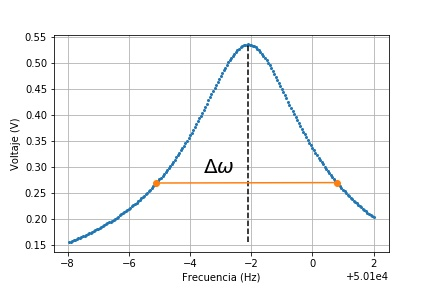
\includegraphics[width=\linewidth]{frecVSampC-cam.jpg}
\caption{Detalle de la campana de resonancia, donde la l\'inea punteada indica el voltaje m\'aximo y la l\'inea horizontal indica los puntos para los cuales el voltaje m\'aximo se reduce a la mitad.}
\label{fig:detalleRESamp}
\end{figure}


\begin{figure}[H]
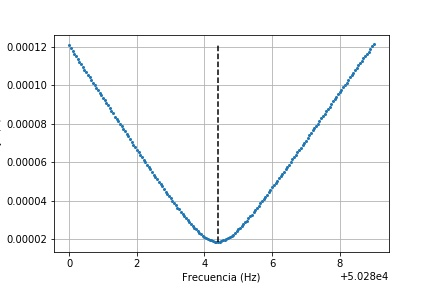
\includegraphics[width=\linewidth]{minimo.jpg}
\caption{Detalle del intervalo donde se produce la antirresonancia indicada por la l\'inea punteada.}
\label{fig:detalleANTamp}
\end{figure}

El \'ultimo m\'etodo que utilizamos consisti\'o en analizar la fase en funci\'on de la frecuencia, considerando que cuando la fase llega a cero de forma descendente corresponde a la fase en la frecuencia de resonancia y que cuando la fase pasa por cero de forma ascendente es que corresponde a la frecuencia de antirresonancia. Se obtuvo que la frecuencia de resonancia es $\omega_{r}$ = (50097,25 $\pm$ 0,05) Hz y que $\omega_{a}$ = (50284,65 $\pm$ 0,05) Hz, en la Figura \ref{fig:fase} se ve la curva completa mientras que en las Figuras \ref{fig:bajada} y \ref{fig:subida} se ven en detalle los puntos donde la diferencia de fase pasa por cero. 

\begin{figure}[H]
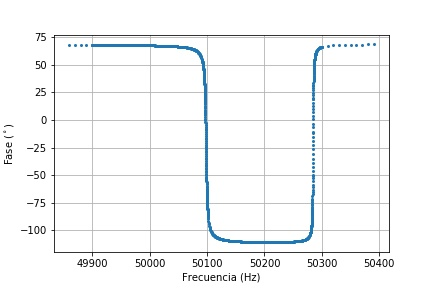
\includegraphics[width=\linewidth]{AMPvsFASE.jpg}
\caption{Diferencia de fase entre la se\~nal de entrada al piezoel\'ectrico y la se\~nal de salida con respecto a la frecuencia.}
\label{fig:fase}
\end{figure}

\begin{figure}[H]
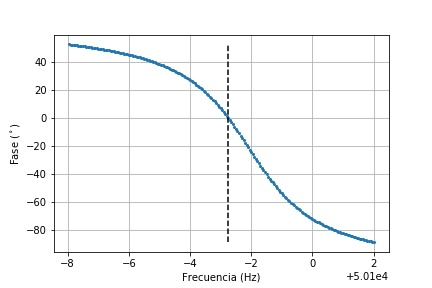
\includegraphics[width=\linewidth]{bajada.jpg}
\caption{Detalle de la diferencia de fase en el intervalo donde se produce la resonancia indicada por la l\'inea punteada.}
\label{fig:bajada}
\end{figure}

\begin{figure}[H]
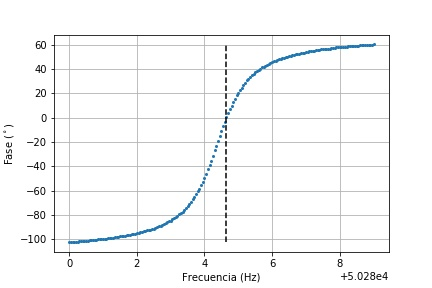
\includegraphics[width=\linewidth]{subida.jpg}
\caption{Detalle de la diferencia de fase en el intervalo donde se produce la antirresonancia indicada por la l\'inea punteada.}
\label{fig:subida}
\end{figure}

Para obtener $\Delta \omega$ se calcularon las frecuencias para las cuales la amplitud m\'axima se habia reducido a la mitad, figura \ref{fig:detalleRESamp}, eso nos di\'o una idea del ancho de la campana $\Delta \omega$ = (5,90 $\pm$ 0,01) Hz. Si comparamos el valor de la frecuencia de resonancia con el ancho de la campana obtenemos el factor de m\'erito, el cual cuanto m\'as grande es, nos indica que m\'as aguda es la campana y que por lo tanto el material es m\'as \'util como resonador en una frecuencia espec\'ifica; en este caso se encontr\'o que el factor de m\'erito es $Q$ = 8491 $\pm$ 5.

Los par\'ametros del circuito que modela el comportamiento del piezoel\'ectrico fueron determinados mediante las ecuaciones (\ref{eq:transferenciar}), (\ref{eq:merito}), (\ref{eq:wr}) y (\ref{eq:wa}), obteni\'endose que la resistencia es $R$ = (13,65 $\pm$ 0,09) K$\Omega$, la inductividad $L$ = (3161 $\pm$ 5) H, la capacitancia es $C$ = (0,126 $\pm$ 0,004) pF; y que la capacitancia producida por la capa de oro que envuelve al piezoel\'ectrico es de $C_{2}$ = (16,9 $\pm$ 0,5) pF.

%------------------------------------------------

\section{Conclusiones}

Se puede observar que los distintos m\'etodos para determinar la frecuencia de resonancia var\'ian en d\'ecimas de Hz, por lo cual consideramos que la experiencia tuvo bastante precisi\'on pues se trabaj\'o con frecuencias del \'orden de los kHz; incluso en un primer barrido manual con el osciloscopio. \\

Sobre la frecuencia de antirresonancia pudimos notar que es preciso un instrumento lo bastante sensible como para poder determinarla, pues el barrido que se realiz\'o con el osciloscopio registraba bastante ruido por lo que no se pudo trabajar con esos datos para determinar dicha frecuencia, mientras que con los datos obtenidos con el amplificador lock-in se pudo obtener un perfil de la curva de voltaje mucho m\'as limpio en comparaci\'on al del osciloscopio y m\'as aun tomando en cuenta el registro de la diferencia de fase que nos permiti\'o el amplificador. \\

El alto factor de m\'erito que obtuvimos nos indica que la campana es bastante aguda, es decir que el ancho de la campana es peque\~no en comparaci\'on a la altura; por lo cual concluimos que el ancho de banda en el cual resuena material piezoel\'ectrico es m\'as estrecho, o visto de otra manera, posee una baja tasa de p\'erdida de energ\'ia en relaci\'on a la almacenada por el mismo.

%----------------------------------------------------------------------------------------
%	REFERENCE LIST
%----------------------------------------------------------------------------------------
\newpage
\begin{thebibliography}{99} % Bibliography - this is intentionally simple in this template


\bibitem{eq:oderlc} R. K. Nagle, E. B. Saff, A. D. Snider, \textit{Ecuaciones diferenciales y problemas con valores en la frontera}, $4^{ta}$ edici\'on, Pearson Educaci\'on M\'exico, 2005, p\'ag. 285
\bibitem{eq:props} http://materias.df.uba.ar/labo4Ba2016c1/files/2014/03/Piezo.pdf 
 
\end{thebibliography}


%----------------------------------------------------------------------------------------

\end{document}